
\section{Example: A regional model of the Jakobshavn outlet glacier}\label{sec:jako} \index{Jakobshavn} \index{PISM!regional model example}

\optsection{Jakobshavn}

Jakobshavn Isbrae is a fast-flowing outlet glacier in western Greenland that drains approximately 7\% of the area of the Greenland ice sheet, and which has experienced a large acceleration following the loss of its floating tongue in the 1990s \cite{JoughinAbdalatiFahnestock}, an event which seems to have been driven by warmer ocean temperatures \cite{Hollandetal2008}.  Because it is thick, it has a steep surface slope, its flow is significantly defined by bedrock topography, and it has a thick layer of low viscosity temperate ice at its base \cite{Luethietal2009}, this outlet glacier is quite different from the cold, shallow ice streams of West Antarctica \cite{TrufferEchelmeyer}.
 
This Section describes the steps, and the scripts in directory \texttt{examples/jako/}, needed to build a PISM regional model of this outlet glacier.  The same strategy will work for others.  In part, the goal is to allow modest-size computers to run high resolution models, and also large ensembles.\footnote{PISM can do 1km runs for the whole Greenland ice sheet, as shown in this \href{http://www.pism-docs.org/wiki/doku.php?id=news:first1km}{news item}, but you certainly need a supercomputer for that!}  On the other hand, additional data may be available for individual outlet glaciers, and additional model-based analysis is a natural goal.

\index{CReSIS bedrock topography for Jakobshavn}
The geometric data is the SeaRISE 1 km dataset for the whole Greenland ice sheet, which also contains bedrock topography from recent CReSIS radar observations in the Jakobshavn area (\small \url{http://websrv.cs.umt.edu/isis/index.php/1km_Greenland_data_set}\normalsize).  We also use the SeaRISE 5 km data set which has surface mass balance from a atmospheric climate model \cite{Ettemaetal2009}.

\begin{figure}[ht]
  \centering
  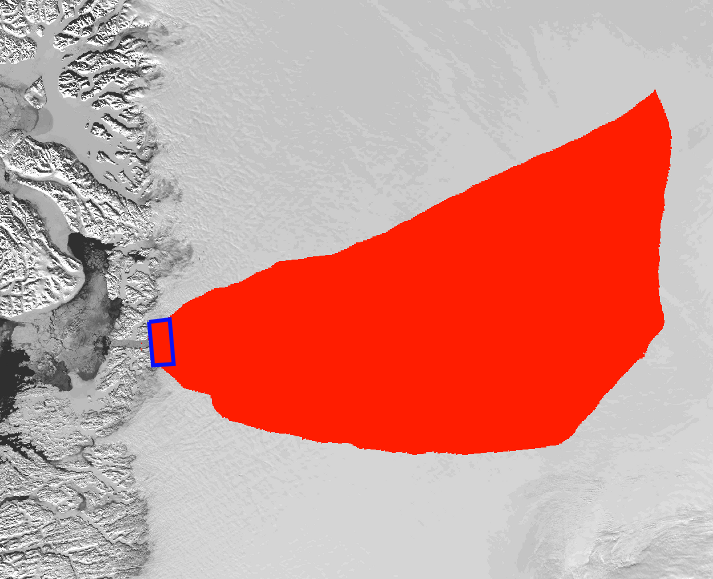
\includegraphics[height=2.1in,keepaspectratio=true]{jako-ftt-mask} \, 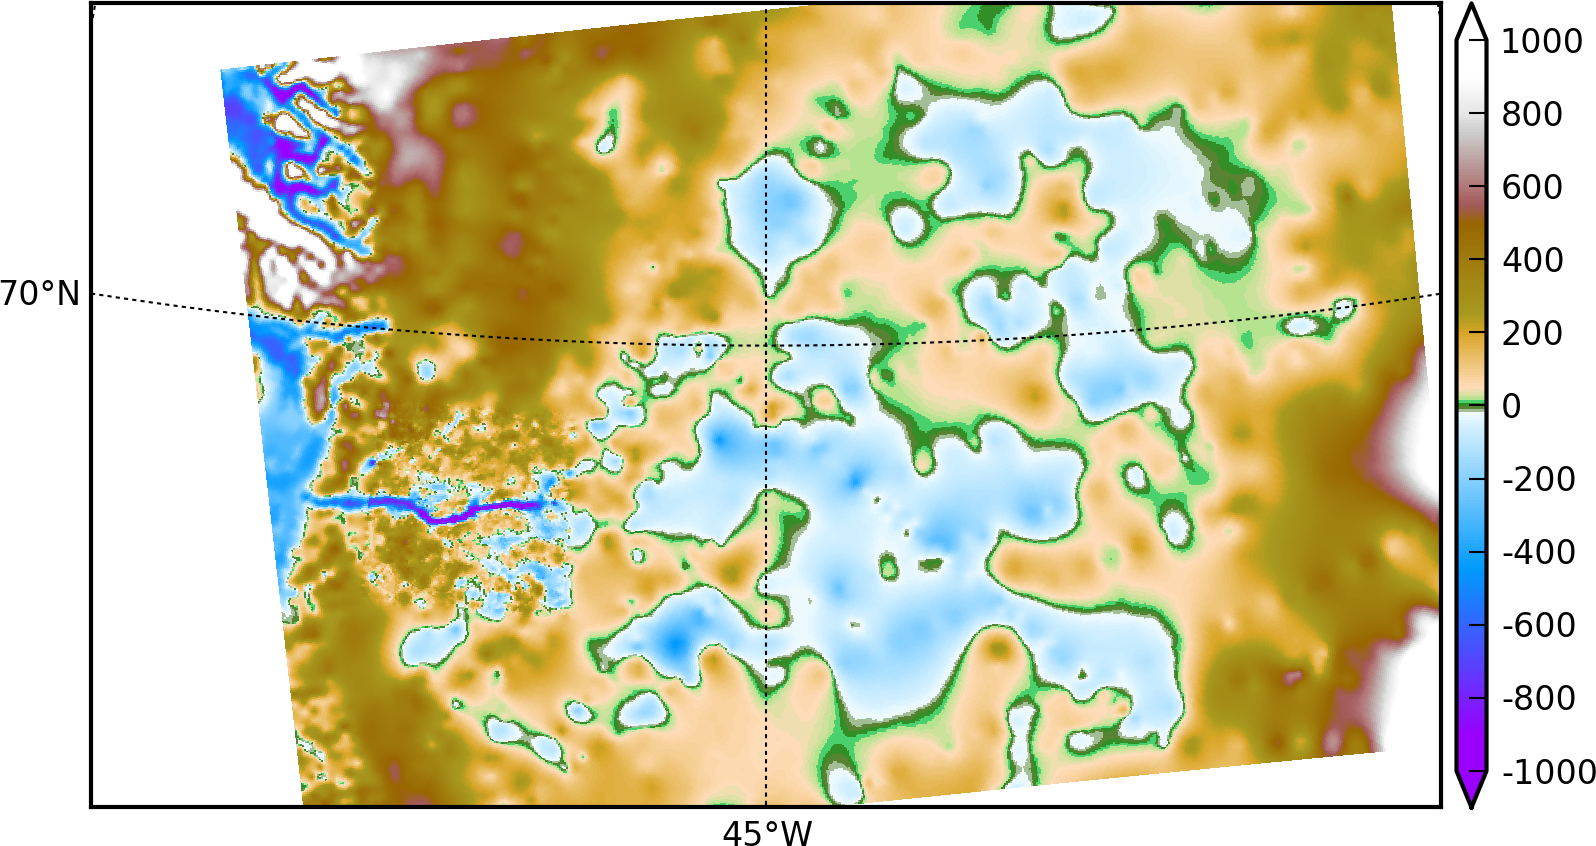
\includegraphics[height=2.1in,keepaspectratio=true]{jako-topg}
  \caption{The Jakobshavn outlet glacier model in this section uses a \texttt{regional-tools} Python script to compute a drainage basin mask from the ice surface elevation (left; Modis background), and starting from a user-identified terminus rectangle (blue).  The regional model benefits from high-resolution bedrock topography in the vicinity of the Jakobshavn fjord (right; scale in meters a.s.l.).}
  \label{fig:jako-basin-topg}
\end{figure}

A regional ice flow model generally needs boundary conditions.  For this we use a 5 km whole ice sheet spun-up model state from PISM, exactly of the type described in Section \ref{sec:start} of this manual.  You can generate the file by running scripts from that Section, or you can download the NetCDF file itself from the PISM website; in fact this download occurs automatically if you run the scripts below.

\index{PISM!pismo executable for outlet glaciers}
\index{regional-tools}
This example in this Section also demonstrates the outlet-glacier-mode PISM executable \texttt{pismo}, and it demonstrates a Python drainage-basin-delineation tool \texttt{regional-tools}, also by the PISM authors, which can be downloaded.

\subsection*{Get the drainage basin delineation tool}
First, get the Python drainage basin generator (using \texttt{git}) and set it up as directed in its \texttt{README.md}.  Then come back to the \texttt{examples/jako/} directory and link to the tool.  Here is the quick summary of these actions:
\begin{quote}\small
\begin{verbatim}
    $ cd ~/usr/local/                                      # the location you want
    $ git clone https://github.com/pism/regional-tools.git
    $ cd regional-tools/
    $ python setup.py install                              # add "--user" to build locally
    $ cd ~/pism/examples/jako/
    $ ln -s ~/usr/local/regional-tools/pism_regional.py .  # symbolic link to tool
\end{verbatim}
\normalsize\end{quote}
To see a description of the drainage basin tool itself, and a bit on how it
works, see \url{https://github.com/pism/regional-tools}.

\subsection*{Preprocess data and whole ice sheet model results}
Next we use a script \texttt{preprocess.sh} that downloads and cleans the 1 km SeaRISE data, an 80 Mb file called \texttt{Greenland1km.nc}.\footnote{If this file is already present then no actual download occurs, and preprocessing proceeds.  So do not worry about download time if you need to preprocess again.  The same comment applies to other downloaded files in this manual.}

The script also downloads the SeaRISE 5 km data set \texttt{Greenland_5km_v1.1.nc}, which contains the surface mass balance model result from RACMO, a field not present in the 1km data set.  If you have already run the example in the first section of this \emph{Manual}, then you already have this file and you can link to it to avoid downloading:
\begin{quote}\small
\begin{verbatim}
    $ ln -s ../searise-greenland/Greenland_5km_v1.1.nc
\end{verbatim}
\normalsize\end{quote}

Finally, the same script also downloads a pre-computed 5 km grid PISM model result \texttt{g5km_0_ftt.nc} for the whole ice sheet.  This is a 1.3Gb file so there may be some delay.  (You can also generate it yourself by running the example in the first section of this \emph{Manual} with its maximum resolution choices, but a supercomputer is recommended for that.)  This download provides the boundary conditions, and the thermodynamical initial condition, for the regional flow model we are building.

So now let's actual run the preprocessing script:
\begin{quote}\small
\begin{verbatim}
    $ ./preprocess.sh
\end{verbatim}
\normalsize\end{quote}
Files \texttt{gr1km.nc}, \texttt{g5km_climate.nc}, and \texttt{g5km_bc.nc} will appear.  These can be examined in the usual ways, for example:
\begin{quote}\small
\begin{verbatim}
    $ ncdump -h gr1km.nc                   # view metadata
    $ ncview gr1km.nc                      # view fields
\end{verbatim}
\normalsize\end{quote}
Note specifically that the boundary condition file \texttt{g5km_bc.nc} contains thermodynamical spun-up variables (\texttt{enthalpy,bmelt,bwat`}) and boundary values for the sliding velocity (\texttt{u_ssa_bc,v_ssa_bc}), which have been extracted from \texttt{g5km_0_ftt.nc}.

None of the above actions is specific to Jakobshavn, though all are specific to the Greenland ice sheet.  If your goal is to build a regional model of another outlet glacier in Greenland, then you may be able to use \texttt{preprocess.sh} immediately.  Note, however, that the SeaRISE 1 km data set only has recent CReSIS bed topography data for the vicinity of the Jakobshavn outlet, and it is otherwise just BEDMAP.  Because outlet glacier flows are bed-topography-dominated, additional effort may be needed to give good models.


\begin{comment}


\subsection*{Extract region for modeling}

We are going to extract a "drainage basin mask" from the 1 km surface
elevation data.  The outline of the flow into the outlet glacier we want to
model can be determined by the gradient flow from the surface elevation.
`pism_regional.py` will identify the upstream area, the drainage basin in the
sense of the surface gradient flow, into a chosen "terminus rectangle".
Within this masked drainage basin we will apply all physics in the PISM model
but outside this basin we will apply simplified models
or use precomputed whole ice sheet results as boundary conditions.

So we use the script `pism_regional.py` from `regional-tools` (see above)q
on `gr1km.nc` (created above):

    $ python pism_regional.py

Running the script opens a graphical user interface
(GUI) which allows you to select a small rectangle around the flux gate or
fjord which is the terminus of the outlet glacier you want to model.

\subsubsection*{To use the GUI}  Select `gr1km.nc` to open.  Once the topographic map appears
in the Figure 1 window, you may zoom enough to see the general outlet glacier
area.  Then select the button `Select terminus rectangle`.
Now use the mouse to select a small rectangle around the Jakobshavn
terminus (calving front).  (<em>At this stage you can choose any other
terminus/calving front and put a small rectangle around it!</em>)
Once you have a highlighted rectangle, select a `border width` of at
least 50 cells.  (<em>This suggestion is somewhat Jakobshavn-specific.
The intention is to have an ice-free western boundary on the computational
domain for our modeled region.</em>)

Then click `Compute the drainage basin mask`.  Because this is a large data set
there will be some delay.  (<em>A parallel computation is done.</em>)

Finally click `Save the drainage basin mask` and save with your
preferred name; we will assume here that it is `jakomask.nc`.  Then quit.  You
can look at the result with `ncview`:

    $ ncview -minmax all jakomask.nc

\subsubsection*{Re-creating the region mask if needed} For repeatability the rest
of this `README.md` assumes a particular
choice of region.  That is, you can skip the GUI usage above and run

    $ python pism_regional.py -i gr1km.nc -o jakomask.nc -x 360,382 -y 1135,1176 -b 50

The options `-x A,B -y C,D` identify the grid indices of the corners of the
terminus rectangle.  Thus this command also generates the file `jakomask.nc`
used in the rest of the script.

Such a step is exactly what is needed to have more precise control over the
identification of a terminus rectangle.  You may need to re-create the region
with slight modifications, for instance.  For more options:

    $ python pism_regional.py --help


\subsection*{Cut out the region from each whole ice sheet data set}

We still need to "cut out" the modeled region we want from the whole sheet data
sets `gr1km.nc` and `g5km_bc.nc`.  (The coarse grid climate data `g5km_climate.nc`
does not need this action because PISM's coupling code can already handle all
needed interpolation/subsampling for such climate data.)

You may have noticed that the text output from `pism_regional.py` includes a
cutout command which appears as a global attribute of jakomask.nc.  Get it this way:

    $ ncdump -h jakomask.nc |grep cutout

Copy and run the command that appears in the string `cutout`, something like

    $ ncks -d x,299,918 -d y,970,1394 gr1km.nc jako.nc

This command is applied to both the 1km Greenland data file and the
mask file, so modify the command to work on the mask also, and note option
`-A` for append:

    $ ncks -A -d x,299,918 -d y,970,1394 jakomask.nc jako.nc

Now look at `jako.nc`:

    $ ncview -minmax all jako.nc

This file is the full geometry data ready for a regional model.  The field
`ftt_mask` has an identified drainage basin, outside of which we
will not use a full model, but use simplified time-independent boundary
conditions instead.  Specifically, outside of the `ftt_mask` area we will
essentially keep the initial thickness, while inside the `ftt_mask` area all
fields will evolve normally.

All of the above steps are accomplished in one script,

    $ ./quickjakosetup.sh

Running this takes about a minute on a fast laptop.


\subsection*{Spinning-up the regional model on a 5km grid}

To run PISM we will need to know the size of the 1km grid in jako.nc.  Do this:

    $ ncdump -h jako.nc |head
    netcdf jako {
    dimensions:
	  y = 425 ;
	  x = 620 ;
	...

The grid has spacing of 1 km, so our region is a 620 km by 425 km rectangle.
A 2km resolution, century-scale model run on this Jakobshavn region is
achievable on a desktop machine, with a bit of patience, and that is our goal below.
A 5km resolution run, which is the resolution of the 5km whole ice sheet state
which was computed on a supercomputer, is definitely achievable on a
desktop or laptop, and that is what we do first.



The whole ice sheet model fields in `g5km_bc.nc`, which is restricted to the 
regional grid as the initial state of the regional model, may or may not,
depending on modeler intent, be spun-up adequately for the purposes of the
regional model.  (For instance, the intention may be to study equilibrium states
with model settings special to the region.)  Here we assume that more
spin-up is needed.  We will get first an equilibrium 5km model, and then do a
century run of a 2km model based on the equilibriated 5km result.
(Determining "equilibrium" requires a decision, of course.  A standard
satisfied here is that the ice volume in the region changes by less than 0.1
percent in the final 100 model years.  See `ivol` in `ts_spunjako_0.nc` below.)

Quick calculations for the 5km grid, e.g. by calculations
`620/5 + 1` and `425/5 + 1`, suggest `-Mx 125 -My 86`.
So now we do a basic run using 4 MPI processes:

    $ ./spinup.sh 4 125 86 >> out.spin5km &

You can read the script, and watch the run, while it runs:

    $ less spinup.sh
    $ less out.spin5km

The run takes about 10 processor-hours.   <!-- 9.12 proc-hours on bueler-lemur -->
The run produces three files which can be viewed with `ncview`:
`spunjako_0.nc`, `ts_spunjako_0.nc`, and `ex_spunjako_0.nc`.

Some comments on the run are appropriate.
The run uses `-boot_file` on `jako.nc`.  A modestly-fine vertical
grid (20 m spacing) is chosen.

There is option `-no_model_strip 10` asking
`pismo` to put a 10km strip around edge of the computational domain wherein
some variables will be held fixed.  Specifically the thermodynamical spun-up
variables `enthalpy`,`bmelt`,`bwat` from `g5km_bc.nc` are held fixed and used
as boundary conditions for the conservation of energy model in the strip.
Additionally, Dirichlet boundary conditions `u_ssa_bc`,`v_ssa_bc` are read
for the sliding stress balance (the SSA) from the same file.

(<em>An alternative is to have the enthalpy and other thermodynamical variables
not spun-up at all in the strip, which would happen if options `-regrid_...`
were not used.  However, the resulting not-very-realistic ice temperatures and
softness/hardness is advected inward. An alternative for the SSA boundary
conditions is to have zero velocity in the `no_model_strip`, but the velocity
tangent to the north and south edges of the strip is significantly nonzero
in fact.  Thus, generally the regridding techniques used here are recommended
for regional modeling.</em>)

The calving front of the glacier is handled by the following options combination:
`-ocean_kill file.nc -cfbc -kill_icebergs`.  This choice uses the present-day
ice extent to determine the location of the calving front, but it then applies
the PIK mechanisms for the stress boundary condition at the calving front
(`-cfbc`) and it uses `-kill_icebergs` to eliminate any stray floating pieces
of ice for which stress balances are indeterminant (ill-posed).


\subsection*{Century run on a 2km grid}

Here is a 100 year run on a 2km grid, starting from the final state generated
by the 5km run above:

    $ ./century.sh 4 311 213 spunjako_0.nc >> out.2km_100a &

This run requires about 6 Gib of memory.  It produces a file almost immediately,
namely `jakofine_short.nc`, and then restarts from it.  (This is explained by the
need to regrid fields first from the result of the previous 5 km regional run,
i.e. from `spunjako_0.nc`, and then to "go back" and regrid the SSA boundary
conditions from the 5 km whole ice sheet results, i.e. from the file
`g5km_bc.nc`.)  At the end of the run the final file `jakofine.nc` is produced,
along with a time-series result file `ts_jakofine.nc` with monthly scalar time-
series, and a spatial time-dependent result file `ex_jakofine.nc`.  The latter
is a source of simple "movies" of the simulation.

The above `century.sh` run takes about 20 processor-hours. <!-- 17.77 proc-hours on bueler-lemur -->

\subsection*{Plotting the results}

FIXME: To visualize the surface speed at the end of the 2km run, do

    $ basemap-plot.py --singlerow -v csurf -o csurf.png jakofine.nc

To choose a colormap add option \verb|--colormap ~/PyPISMTools/colormaps/Full_saturation_spectrum_CCW.cpt| or similar.

\end{comment}


